\paragraph{Transformers} Transformers \parencite{vaswani2017attention} are a class
of neural networks which map an input sequence to an output sequence of the same
length and utilize a mechanism known as ``self-attention.'' Self-attention maps
the $i^\Th$ element of the input sequence to a key vector $k_i$, a value vector
$v_i$, and query vector $q_i$. The output of self-attention is a weighted sum of
the value vectors:
\begin{align}
    \text{Attention}\left(q_i, k, v\right) = \sum_j\text{softmax}\left(q_i k_j/\sqrt{D}\right)v_j
\end{align}
where $D$ is the dimensionality of the vectors. The softmax is applied accross
the inputs so that $\sum_j\text{softmax}\left(q_i k_j/\sqrt{D}\right) = 1$. A
typical transformer applies this self-attention operation multiple times,
interspersing linear projections and layer-norm operations between each
application. A \textit{causal} transformer applies a mask to the attention
operation which prevents the model from attending from the $i^\Th$ element to
the $j^\Th$ element if $i < j$, that is, if the $j^\Th$ element appears later in
the sequence.


\paragraph{Policy Iteration}
Policy iteration is a technique for improving a policy in which one estimates
the values for the current policy and then chooses actions greedily with respect
to these value estimates. This yields a new policy which is at least as good as
the original policy according to the policy improvement theorem (assuming that
the value estimates are correct). This process may be repeated indefinitely
until convergence. To choose actions greedily with respect to the value
estimates, there must be some mechanism for estimating value conditioned not
only on the current state and policy but also on an arbitrary action. The
``greedy'' action choice corresponds to the action with the highest value
estimate. Policy iteration is possible if our value estimates are unbiased for
any state-action pair and for the current policy.

\paragraph{Algorithm Distillation}
Algorithm Distillation \parencite{laskin2022context} is a method for distilling the
logic of a source RL algorithm into a causal transformer. The method assumes
access to a dataset of ``learning histories'' generated by the source algorithm,
which comprise state, action, reward sequences spanning the entire course of
learning, starting with initial random behavior and ending with fully optimized
behavior. The transformer is trained to predict actions given the entire history
of behavior or some large subset of it. Optimal prediction of these actions
requires the model to capture not only the current policy but also the
improvements to that policy by the source algorithm. Auto-regressive rollouts of
the distilled model, in which actions predicted by the model are actually used
to interact with the environment and then cycled back into the model input,
demonstrate improvement of the policy without any adjustment to the model's
parameters, indicating that the model does, in fact, capture some policy
improvement logic from the source algorithm.

\section{Method}
In this section, we describe the details of our proposed algorithm, which we
call In-Context Model-Based Planning (ICMBP). We assume a dataset of $N$
trajectories generated by interactions with an environment:
\begin{align}
    \Dataset :=
    \left\{
    \Tuple
    { \Obs^n_0 }
    { \Act^n_0 }
    { \Rew^n_0 }
    { \Ter^n_0 }
    { \dots }
    { \Obs^n_T }
    { \Act^n_T }
    { \Rew^n_T }
    { \Ter^n_T }
    \sim \Tuple {\Policy}{\Task}_n
    \right\}_{n=1}^N
\end{align}

with $\Obs^n_t$ referring to the $t^\Th$ observation in the $n^\Th$
trajectory, $\Act^n_t$ to the $t^\Th$ action, $\Rew^n_t$ to the $t^\Th$
reward, and $\Ter[t](n)$ to the $t^\Th$ termination boolean. Each trajectory
corresponds with a single task $\Task$ and a single policy $\Policy$, but the
dataset contains as many as $N$ tasks and policies. We also introduce the
following nomenclature for trajectory histories:

\begin{align}
    \History^n_t :=
    \Set
    { \Act^n_{t-C} }
    { \Rew^n_{t-C} }
    { \Ter^n_{t-C} }
    { \Obs^n_{t-C+1} }
    { \dots }
    { \Act^n_{t-1} }
    { \Rew^n_{t-1} }
    { \Ter^n_{t-1} }
    { \Obs^n_{t} }
    \locallabel{eq:history}
\end{align}

where $C$ is a fixed hyperparameter.

\subsection{Model Training}
Given such a dataset, we may train a
world-model with a negative log likelihood (NLL) loss:

\begin{align}
    \Loss[\theta] :=
    -\sum_{n=1}^N\sum_{t=1}^{T-1}
    \log \Prob[\theta]
    [ \Act^n_t ]
    [ \History^n_t ] +  \log \Prob[\theta]
    [ \Rew^n_t, \Ter^n_t, \Obs^n_{t+1} ]
    [ \History^n_t, \Act^n_t ]
\end{align}

In this work we implement $\Prob_\theta$ as a causal transformer. For
action-prediction $\Prob_\theta [ \Act^n_t ] [ \History^n_t ]$, the inputs
comprise chronological
$\Tuple{\Act^n_{i-1}}{\Rew^n_{i-1}}{\Ter^n_{i-1}}{\Obs^n_i}_{i=t-C}^t$ tuples.
Each index of the transformer comprises one such tuple, with each component of
the tuple embedded and the embeddings concatenated. For the other predictions
$\Prob_\theta [ \Rew^n_t, \Ter^n_t, \Obs^n_{t+1} ] [ \History^n_t, \Act^n_t ]$,
we use the same procedure but rotate each tuple such that index $i$ corresponds
to $\Tuple{\Rew^n_{i-1}}{\Ter^n_{i-1}}{\Obs^n_{i-1}}{\Act^n_{i}}$.

\subsection{Downstream Evaluation}
\begin{figure}[tb]
    %  \vspace*{-2.5em}
    % \begin{minipage}{0.6\textwidth}
    \begin{algorithm}[H]
        \caption{Estimating Q-values with monte-carlo rollouts.}
        \locallabel{alg:rollout}
        \begin{algorithmic}[1]
            \Function{Q}{$\History, \Act$}
            % \State $q \gets 0$\Comment{Initialize Q-estimate.}
            \State $t \gets 0$\Comment{Initialize simulation time.}
            \State $\Act*_{t} \gets \Act$
            \While{termination condition not met}
            \State $\Rew*_{t},\Ter*_{t},\Obs*_{t+1} \sim \Prob_\theta[\cdot][\History, \Act*_{t}]$
            \Comment{Model reward, termination, next observation.}
            \State $\Act*_{t+1} \sim \Prob_\theta[\cdot][\History, \Act, \Rew*_{t}, \Ter*_{t},
                    \Obs*_{t+1}]$
            \Comment{Model action.}
            \State $\History \gets \History \cup \Set {\Rew*_{t}}{\Ter*_{t}}{\Obs*_{t+1}}{\Act*_{t+1}}$
            \Comment{Append predictions to history.}
            % \State $q \gets q + \gamma^t \Rew*_{t}$ \Comment{Update Q-estimate.}
            \State $t \gets t+1$ \Comment{Increment simulation time.}
            \EndWhile
            \State \textbf{return} $\sum_{u=0}^{t} \gamma^{u - 1} \Rew*_u$
            \EndFunction
        \end{algorithmic}
    \end{algorithm}
    % \end{minipage}
    %  \vspace*{-1em}
\end{figure}
Our approach to choosing actions during the downstream evaluation is as follows.
For each action $\Act$ in a set of candidate actions (either our complete action
space or some subset thereof), we compute a state-action value estimate
$\Q*[\History_t][\Act]$, where $\History_t$ is the history defined in
(\localref{eq:history}). We do this by modeling a rollout from the current state
(conditioned on the history $\History_t$) and from $\Act$. Modelling the
rollout is a cycle of sampling values from the model and feeding them back into
the model auto-regressively. First we sample
$\Tuple{\Rew*_t}{\Ter*_t}{\Obs*_{t+1}}$. Based on this prediction, we sample
$\Act*_{t+1}$. Adding this to the input allows us to sample
$\Tuple{\Rew*_{t+1}}{\Ter*_{t+1}}{\Obs*_{t+2}}$, repeating this cycle until some
termination condition is reached. For example, we might terminate the process
once $\Ter*_{i}$ is true, or once the rollout reaches some maximum length.

The final step is to choose an action. Having modelled the rollout, we compute
the value estimate as the discounted sum of rewards in the rollout. See
Algorithm \localref{alg:rollout} for a pseudocode implementation. Repeating this
process of modelling rollouts and computing value estimates for each action in
pool of candidate actions, we simply choose the action with the highest value
estimate: $\arg\max_{\Act \in \Actions} \Q*[\History_t][\Act]$.

\subsection{Policy improvement}
If the downstream task is sufficiently dissimilar to the tasks in the training
dataset, or if the training dataset does not contain optimal policies, then it
is unlikely that the procedure described above will initially yield an optimal
policy. Some method for policy improvement will be necessary.

\paragraph{Policy Iteration}
Our method satisfies this requirement by implementing a form a policy iteration.
To see this, first observe that our model is always trained to map a behavior
history drawn from a single policy to actions drawn from the same policy. A
fully trained model will therefore learn to match the distribution of actions in
its output to the distribution of actions in its input. Since our rollouts are
conditioned on histories drawn from our behavior policy, the rollout policy will
approximately match this policy. Our value estimates will therefore be
conditioned on the current behavior policy.  However, by choosing the action
corresponding to $\arg\max_{\Act \in \Actions} \Q*[\History_{t}][\Act]$, our
behavior policy always improves on the policy on which $\Q*[\History_{t}][\Act]$
is conditioned, a consequence of the policy improvement theorem. Thus, each time
an action is chosen using this $\arg\max$ method, our behavior policy improves
on itself.

Walking through this process step by step, suppose $\Policy^n$ is some policy
that we use to behave. We collect a trajectory containing actions drawn from
this policy. When we perform rollouts, we condition on this trajectory and the
rollout policy simulates $\Policy^n$. Assuming that this simulation is accurate
as well as the world model, our value estimate will be an unbiased monte carlo
estimate of $\Q*[\History_{t}][\Act]$ for any action $\Act$. Then we
act with policy $\Policy^{n+1} := \arg\max_{\Act \in \Actions}
    \Q*[\History_{t}][\Act]$. But $\Policy^{n+1}$ is at least as good as
$\Policy(n)$. Using the same reasoning, $\Policy^{n+2}$ will be at least as good
as $\Policy^{n+1}$, and so on. Note that in our implementation, we perform the
$\arg\max$ at each step, rather than first collecting a full trajectory with a
single policy.

\paragraph{Algorithm Distillation}
Our setting is almost identical to Algorithm Distillation (AD), if we include
the assumption that trajectories include a full learning history. Rather than
competing with AD, our method is actually complementary to it. If the input to our
transformer is a sufficiently long history of behavior, then the rollout policy
will not only match the input policy but actually improve upon it, as
demonstrated in that paper. Then $\Q*$ will actually estimate values for a
policy $\Policy*(n)$ that is at least as good as the input policy $\Policy(n)$.
Then
$$\V^{\Policy^{n+1}} \ge \V^{\Policy*^{n}} \ge \V^{\Policy^{n}}$$
Therefore each step
of improvement actually superimposes the two improvement operators, one from the
$\arg\max$ operator, the other from AD.

\section{Experiments}
\paragraph{Domains}
In this work, we chose to focus on partially observable domains. This ensures
that both the initial policy and the initial model in our downstream domain will
be suboptimal, since the true dynamics or reward function cannot be inferred
until the agent has gathered experience. Recovering the optimal policy will
require policy improvement along side model improvement. Model improvement will
occur as the agent collects experience and the transformer context is populated
with transitions drawn from the current dynamics and reward functions. Policy
improvement relies on the mechanisms detailed in the previous sections. One
hypothesis that our experiments test is whether these learning processes can
successfully happen concurrently.

All of our experiments occur within a discrete, partially observable, $5\times
    5$ grid world. The agent has four actions, up, left, down, right. For each
task, we spawn a key and a door in a random location. The agent receives a
reward of 1 for visiting the key location and then a reward of 1 for
visiting the door. The agent observes only its own position and must infer
the positions of the key and the door from the history of interactions which
the transformer prompt contains. The episode terminates when the agent visits
the door, or after 25 time-steps.


\paragraph{Baselines}
Currently we compare our method with two baselines: vanilla AD and
``Ground-Truth'' ICMBP. The latter is identical to our method, but uses a
ground-truth model of the environment, which is free of error. The comparison
with AD highlights the contribution of the model-based planning component of our
method. The comparison with Ground-Truth ICMBP establishes an approximate upper
bound for our method and distinguishes the contribution of model error to the
RL metrics that we record.

\subsection{Results}
\begin{figure}
    \centering
    \begin{subfigure}{0.35\textwidth}
        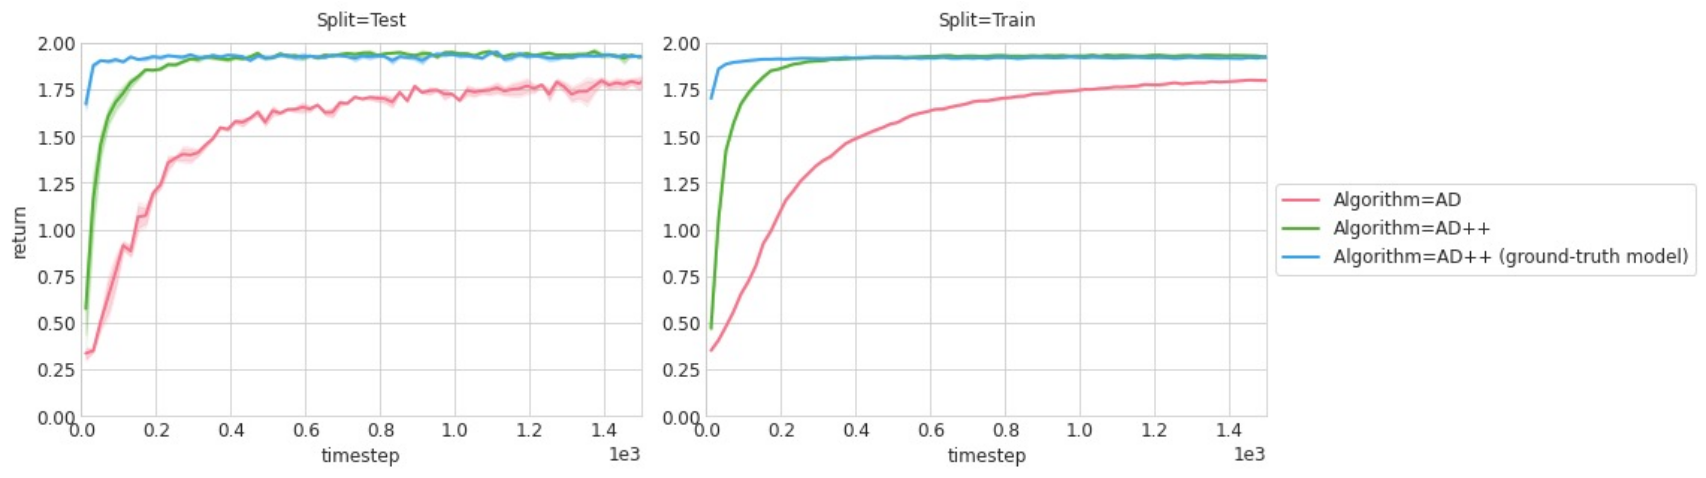
\includegraphics[width=\textwidth]{no-walls}
        \caption{Evaluation on withheld location pairs.}
        \locallabel{fig:no-walls}
    \end{subfigure}
    \hfill
    \begin{subfigure}{0.58\textwidth}
        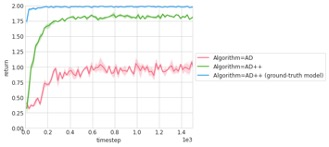
\includegraphics[width=\textwidth]{unseen-goals}
        \caption{Evaluation on fully withheld locations.}
        \locallabel{fig:unseen-goals}
    \end{subfigure}
\end{figure}



\paragraph{Evaluation on Withheld Goals}
In our first experiment, we evaluate the agent on a set of withheld key-door
pairs, which we sample uniformly at random (10\% of all possible pairs) and
remove from the training set. As figure \localref{fig:no-walls} indicates, our
algorithm outperforms the AD baseline both in time to converge and final
performance. We attribute this to the fact that our method's downstream policy
directly optimize expected return, choosing actions that correspond to the
highest value estimate. In contrast, AD's policy only maximizes return by proxy
--- maximizing the probability of the actions of a source algorithm which in
turn maximizes expected return. This indirection contributes noise to the
downstream policy through modeling error. Moreover, we note that our method
completely recovers the performance of the ground-truth baseline, though its
speed of convergence lags behind slightly, due to the initial exploration phase
in which the model learns the reward function through trial and error.

Next, we increase the generalization challenge by holding out key and door
locations entirely, never training the agent source algorithm on keys or doors
in the upper-left four cells of the grid and then placing both keys and doors
exclusively within this region during downstream evaluation. As
figure \localref{fig:unseen-goals} demonstrates, AD generalizes poorly in this setting,
on average discovering only one of the two goals. In contrast, our method
maintains relatively high performance. We attribute this to the fact that our
method learns low-level planning primitives (the reward function), which
generalize better than high-level abstractions like a policy. As we argued in
section \localref{sec:intro}, higher-level abstractions are prone to memorization
since they do not always distill the logic which produced them.


\begin{figure}
    \centering
    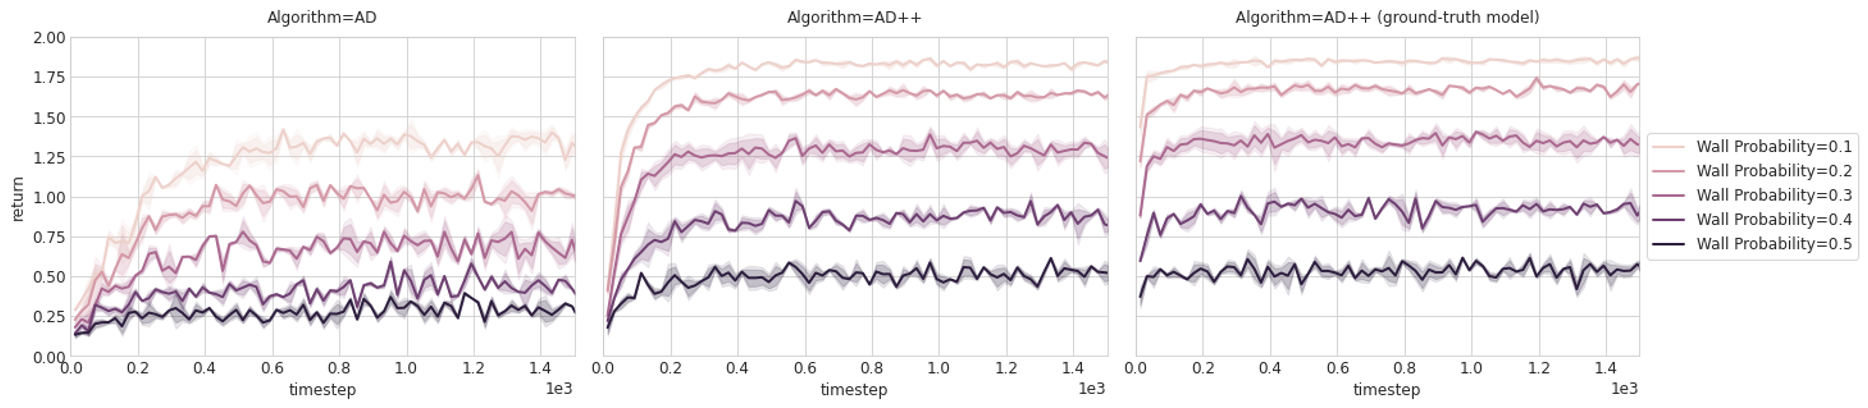
\includegraphics[width=\linewidth]{generalization-to-more-walls-timestep}
    \caption{Generalization to higher percentages of walls.}
    \locallabel{fig:wall-percent}
\end{figure}


\paragraph{Evaluation on Withheld Wall Configurations}
In addition to evaluating generalization to novel reward functions, we also
evaluated our method's ability to generalize to novel dynamics. We did this by
adding walls to the grid world, which obstruct the agent's movement. During
training we placed the walls at all possible locations, sampled IID, with 10\%
probability. During evaluation, we tested the agent on equal or higher
percentages of wall placement. As indicated by figure
\localref{fig:wall-percent}, out method maintains performance and nearly matches
the ground-truth version, while AD's performance rapidly degrades. Again we
attribute this to the tendency of lower-level primitives to generalize better
than higher-level abstractions.

\begin{figure}[b]
    \centering
    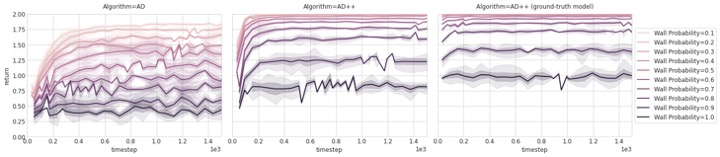
\includegraphics[width=\textwidth]{more-walls-achievable-timestep}
    \caption{Generalization to higher percentages of walls with guaranteed achievability.}
    \locallabel{fig:achievable-wall-percent}
\end{figure}

Because walls are chosen from all possible positions IID, some configurations
may wall off either the key or the door. In order to remove this confounder, we
ran a set of experiments in which we train the agent in the same 10\% wall
setting as before, but evaluate it on a set of configurations that guarantee the
reachability of both goals. Specifically, we generate procedural mazes in which
all cells of the grid are reachable and sample some percentage of the walls in
the maze. As figure \localref{fig:achievable-wall-percent} demonstrates, this
widens the performance gap between our method and the AD baseline.

\paragraph{Model Accuracy}
In order to acquire a better understanding of the model's ability to in-context
learn, we plotted model accuracy in the generalization to 10\% walls setting.
Note that while the percentages of walls in the training and evaluation setting
are the same, the exact wall placements are varied during training and the
evaluation wall placements are withheld, so that the model must infer them from
context. In figure \localref{fig:model-accuracy}, we measure the model's
\begin{wrapfigure}{l}{0.6\textwidth}
    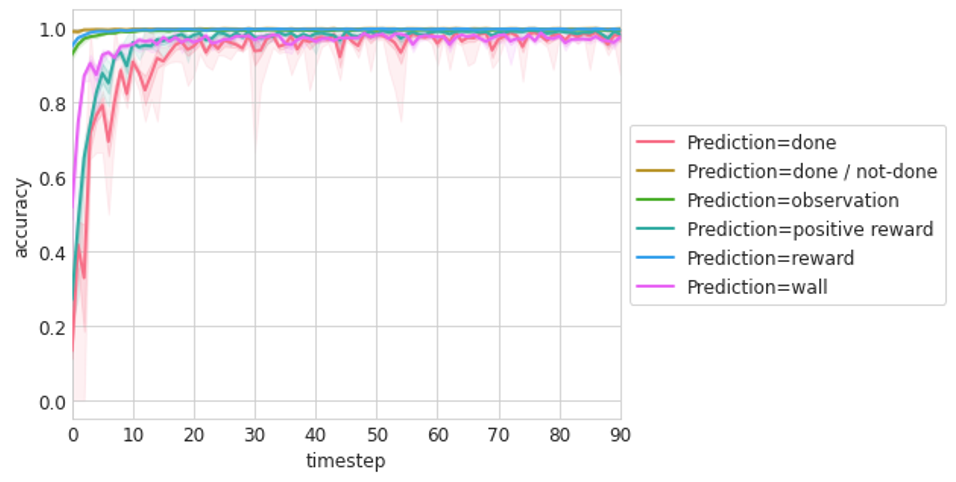
\includegraphics[width=0.6\textwidth]{model-accuracy}
    \caption{Evaluation with no walls.}
    \locallabel{fig:model-accuracy}
\end{wrapfigure}
prediction accuracy of termination signals (labeled ``done / not done''), of
next observations (labeled ``observation''), and of rewards (labeled
``reward''). These predictions start near optimal, since the agent can rely on
priors, that most timesteps do not terminate, that most transitions result in
successful movement (no wall), and that the reward is 0. However, we also
measure prediction accuracy for these rare events: the line labeled ``done''
measures termination-prediction accuracy exclusively on terminal timesteps; the
``positive reward'' line measures reward-prediction accuracy exclusively on
timesteps with positive reward; and the ``wall'' line measures accuracy on
timesteps when the agent's movement is obstructed by a random wall. As figure
\localref{fig:model-accuracy} demonstrates, even for these rare events, the
model rapidly recovers accuracy near 100\%.

\paragraph{Contribution of Model Error to Performance}
\begin{figure}[b]
    \centering
    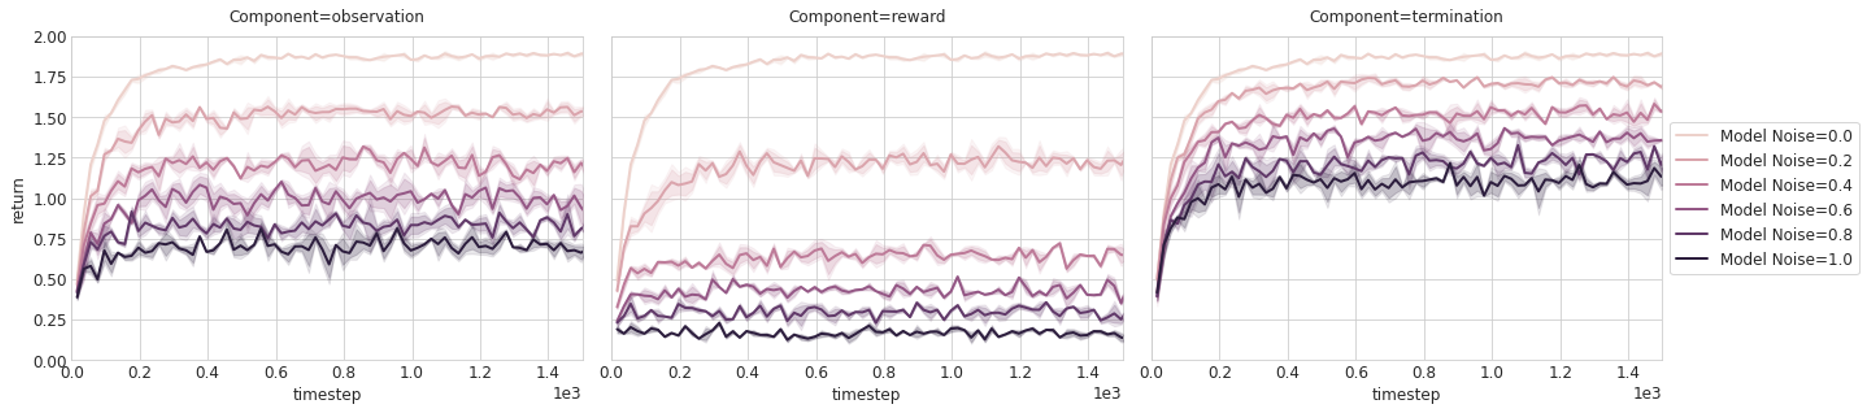
\includegraphics[width=\textwidth]{model-noise}
    \caption{Impact of model error on performance, measured by introducing noise
        into each component of the model's predictions.}
    \locallabel{fig:model-noise}
\end{figure}
While figure \localref{fig:model-accuracy} indicates that our model generally
achieves high accuracy in these simple domains, we nevertheless wish to
understand the impact of a suboptimal model on RL performance. To test this, we
introduced noise into different component of the model's predictions. In figure
\localref{fig:model-noise}, we note that performance is fairly robust to noise
in the termination predictions, but very sensitive to noise in the reward
predictions. Encouragingly, the model is demonstrates reasonable performance
with as much as 20\% noise in the observation predictions. Also, as
\localref{fig:policy-noise} indicates, the method is quite robust to noise in
the action model. We also note that AD's sensitivity to noise in the policy
explains its lower performance in many of the settings previously discussed.

\begin{figure}
    \centering
    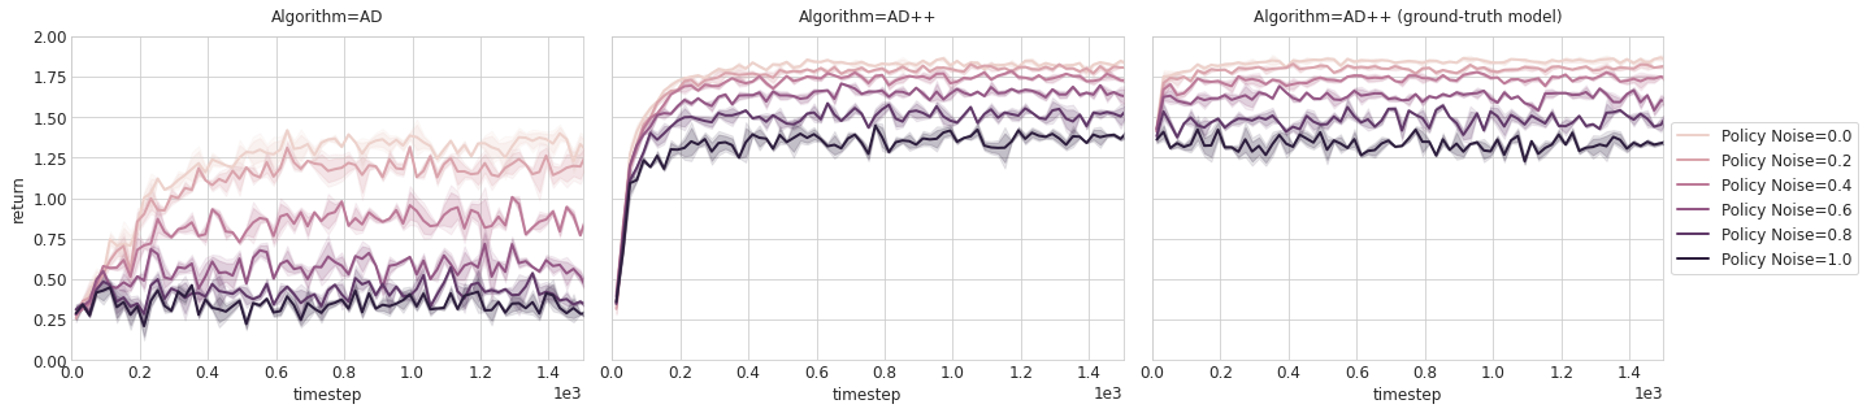
\includegraphics[width=\textwidth]{policy-noise-timestep}
    \caption{Impact of model error on performance, measured by introducing noise
        into each component of the model's predictions.}
    \locallabel{fig:policy-noise}
\end{figure}

\paragraph{Data Scaling Properties}
\begin{figure}[b]
    \centering
    \begin{subfigure}{0.48\textwidth}
        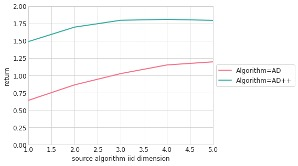
\includegraphics[width=\textwidth]{less-source-data-iid-dimension}
        \caption{Impact of scaling the training data along the IID dimension.}
        \locallabel{fig:scale-source-iid}
    \end{subfigure}
    \hfill
    \begin{subfigure}{0.48\textwidth}
        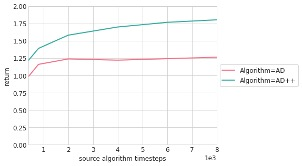
\includegraphics[width=\textwidth]{less-source-data-time-timestep}
        \caption{Impact of scaling the length of training of the source algorithm.}
        \locallabel{fig:scale-source-time}
    \end{subfigure}
\end{figure}
Finally, we examined the impacts of scaling the quantity of data that our model
was trained on. In figure \localref{fig:scale-source-iid}, we scale the quantity
of the training data along the IID dimension, with the $x$-axis measuring the
number of source algorithm histories in the training data scaled according to
the equation $256 \times 2^x$. In figure \localref{fig:scale-source-time}, we
scale the length for which each source algorithm is trained, with the $x$-axis
measuring the number of timesteps of training scaled according to the same
equation. This result was surprising, as we expected AD to be \emph{more}
sensitive to reduced training time, since that algorithm is more dependent on
demonstration of the optimal policy. Nevertheless we note that our method
outperforms AD in all data regimes.

\section{Conclusion}
This chapter presents an approach for combining ICPI with AD. The resulting
method scales to more complex settings than those explored in the previous
chapter. Moreover, the method significantly outperforms vanilla AD in a wide
variety of settings. For the final version of this thesis, we intend to test
this method on more complex domains, especially those involving simulated
robotics. We also intend to evaluate more baselines, especially those from the
traditional meta-learning literature like RL$^2$ \parencite{duan_rl2_2016}.